\documentclass{article}
\usepackage[utf8]{inputenc}
\usepackage[margin=1in]{geometry}
\usepackage{amsfonts}
\usepackage{hyperref}
\usepackage[usenames,dvipsnames]{xcolor}
\usepackage{helvet}
\usepackage{graphicx,wrapfig,lipsum}
\usepackage{enumitem}

\setlength{\parskip}{\baselineskip}
\setlength{\parindent}{0pt}
\definecolor{DarkGreen}{HTML}{013300}
\definecolor{DarkRed}{HTML}{66001B}
\definecolor{DarkBlue}{HTML}{003366}
\renewcommand{\familydefault}{\sfdefault}

\newcommand{\hl}{\textcolor{DarkRed}{\textbf{HL: }}}
\newcommand{\rms}{\textcolor{DarkBlue}{\textbf{RMS: }}}

\title{\textbf{HardwareLogic Interviews Dr. Richard Stallman}}
\author{Joshua Williams}
\date{May 28, 2007}

\begin{document}
\maketitle

HL recently interviewed world-renowned free software developer Dr. Richard Stallman, author of such software as the GNU C Compiler and Emacs. We asked the most hard-hitting questions regarding the free software movement and its ethics$\ldots$ and more.

\begin{itshape}\color{DarkGreen}{``Richard Stallman is the founder of the GNU Project, launched in 1984 to develop the free software operating system GNU. The name `GNU' is a recursive acronym for `GNU's Not Unix'.

GNU is free software: everyone is free to copy it and redistribute it, as well as to make changes either large or small. Non-free software keeps users divded and helpless, forbidden to share it and unable to change it. A free operating system is essential for people to be able to use computers in freedom. Today, Linux-based variants of the GNU system, based on the kernel Linux developed by Linus Torvalds, are in widespread use. There are estimated to be some 20 million users of GNU/Linux systems today.

Richard Stallman is the principal author of the GNU Compiler Collection, a portable optimizing compiler which was designed to support diverse architectures and multiple languages. The compiler now supports over 30 different architectures and 7 programming languages.

Stallman graduated from Harvard in 1974 with a BA in physics. During his college years, he also worked as a staff hacker at MIT Artificial Intelligence Lab, learning operating system development by doing it. He wrote the first extensible Emacs text editor there in 1975. He also developed the AI technique of dependency-directed backtracking, also known as truth maintenance. In January 1984 he resigned from MIT to start the GNU project.

Stallman received the Grace Hopper award for 1991 from the Association for Computing Machinery, for his development of the first Emacs editor. In 1990 he was awarded a Macarthur foundation fellowship, and in 1996 an honorary doctorate from the Royal Institute of Technology in Sweden. In 1998 he received the Electronic Frontier Foundation's pioneer award along with Linus Torvalds. In 1999 he received the Yuri Rubinski award. In 2001 he received a second honorary doctorate, from the University of Glasgow, and shared the Takeda award for social/economic betterment with Torvalds and Ken Sakamura. In 2002 he was elected to the US National Academy of Engineering, and in 2003 to the American Academy of Arts and Sciences. In 2003 he was named an honorary professor of the Universidad Nacional de Ingenieria in Peru, and received an honorary doctorate from the Free University of Brussels. In 2004 he received an honorary doctorate from the Universidad Nacional de Salta, in Argentina.''}\end{itshape} - \href{https://web.archive.org/web/20070621122858/http://www.stallman.org/#urgent}{\color{DarkRed}{Dr. Stallman's Homepage}}

\newpage

\begin{wrapfigure}[10]{l}{5.5cm}
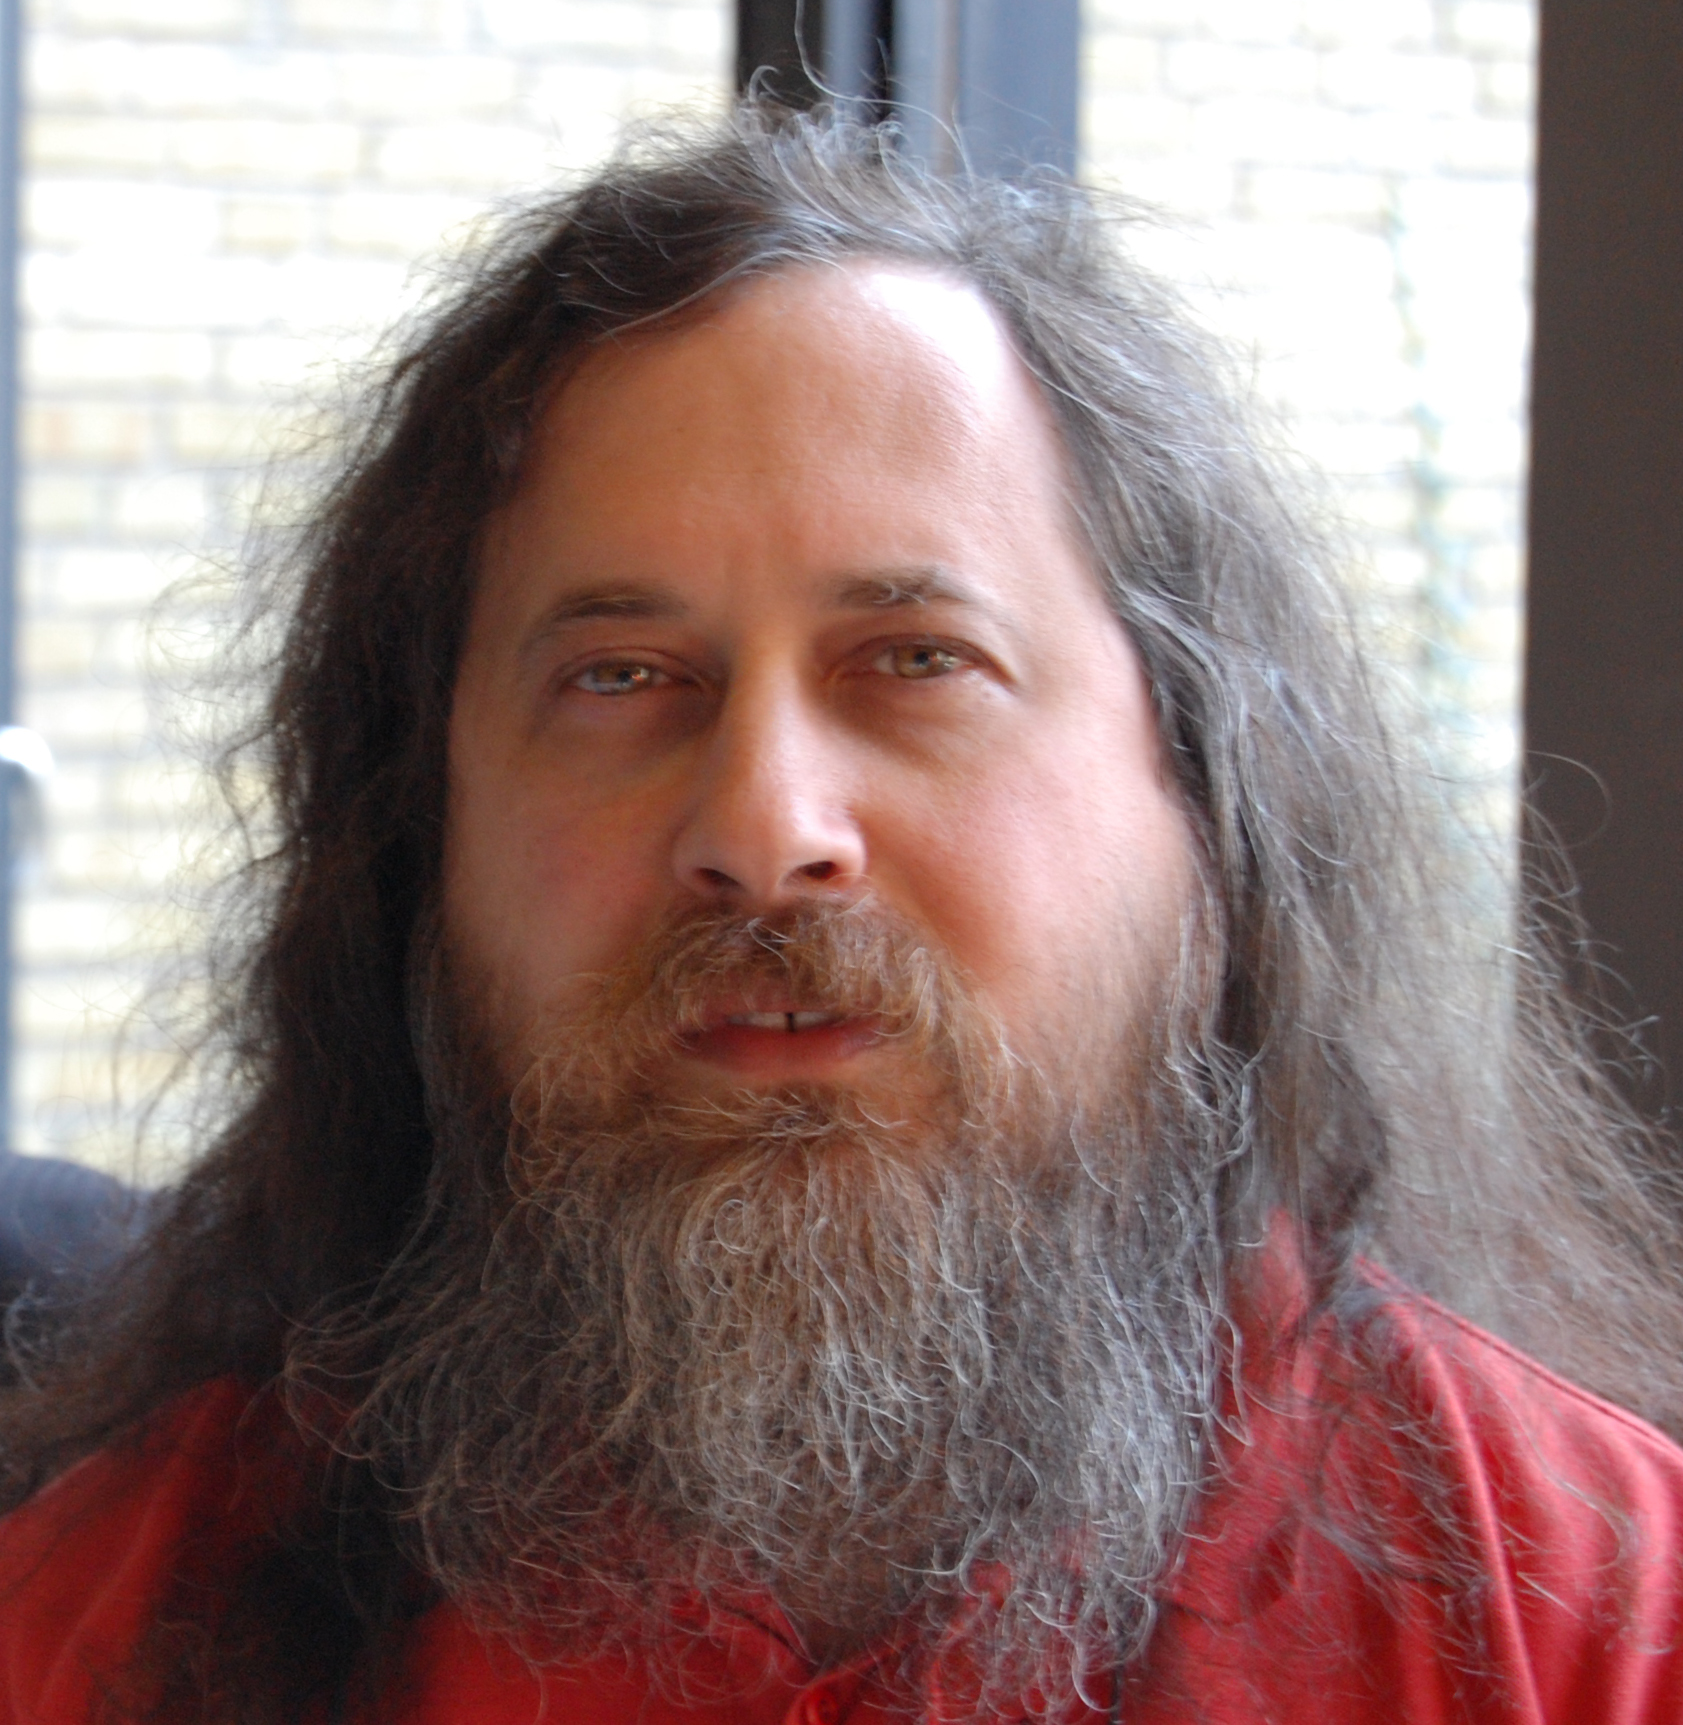
\includegraphics[width=5cm]{rms.jpg}
\end{wrapfigure}
\hl What is free software?

\rms Letting users look at the source code is not enough to be free software (or even to be open source, according to the official definition).  A program is free software if it gives the users these four essential freedoms:
\begin{enumerate}[topsep=0pt, itemsep=0pt]
\setcounter{enumi}{-1}
\item The freedom to run the program, as you wish.
\item The freedom to study the source code and change it so the program does what you wish.
\item The freedom to make and distribute exact copies to others, either commercially or noncommerically, when you wish.
\item The freedom to make and distribute copies of your modified versions to others, either commercially or noncommercially, when you wish.
\end{enumerate}
These are the freedoms that we need in order to have full control of our own computing, and to cooperate in a community. Without them, the developer always more or less has power over the users.

\hl In your speeches, you have often told the story of starting the GNU project in order to provide an alternative to the restrictive, proprietary operating systems. Although you now have a very high reputation for using only free software, obviously, there was a time when this was not possible. Was there a specific turning point when you recognized the need for a move to free software?

\rms I learned to appreciate the free software way of life in the 1970s while working for the MIT Artificial Intelligence Lab, using and developing the Incompatible Timesharing System. Sharing software was our way of life, and we were happy to share our work with anyone who was interested.

Occasional brushes with proprietary software, which made a sharp contrast with my community, showed me the unethical nature of non-free software, and the power that its developers impose on its users. When the old free-software community died, in the early 80s, and its software became obsolete, I realized that the rest of my life would be spent in a shameful and ugly world of proprietary software--unless I did something to change it.

So in 1983 I decided to develop a new free operating system, in order to create a new community of cooperation. Free software, as such, was not new, though little important free software still existed then. What was new was to make a social movement for free software, a movement to put an end to the social problem of proprietary software and give computer users the freedom to cooperate and share.

\hl What is your opinion on proprietary software that is later freed, such as Netscape (AKA Firefox)? Do you believe it would be considered morally right to use this software after it has been freed?

\rms The reason you shouldn't use non-free software is because it tramples your freedom, and (in most cases) requires you to betray your community by promising not to share it. If the program is freed, those reasons no longer apply to it. There is no point holding a grudge against past abuses that have been rectified.

However, in regard to Firefox, I am sad to say that only the source code is free. The Firefox binaries include a non-free module called Talkback, whose sources are not available, and they carry an EULA which is unacceptably restrictive. So these binaries are not free software. This is why the free distributions of GNU/Linux have their own binaries, with names such as Iceweasel and Burningdog, that are made from the free Firefox sources.

\hl It seems that GNU/Linux systems have recently gained very large momentum as a desktop platform. Many see Ubuntu as a large factor for this, due to its ease of use for the average user, especially if they are installing it for the first time in order to dual boot with a Microsoft system. Do you agree with this statement at all?

\rms Improving ease of use is important, but we must not focus on this to the point where we overlook ethical issues. Ubuntu recommends the installation of many non-free programs. Worse, it installs non-free drivers without even informing the user, when it sees hardware that ``needs'' these drivers. To recommend using Ubuntu is to recommend use of non-free software.

I recommend use of the gNewSense distribution, which is based on Ubuntu but is completely free. It is just as easy to use.

\hl People who are new to free software often rely at least partially on restricted software until they find and learn how to use free alternatives. Do you see this transition as a reasonable approach for the average user?

\rms The goal is freedom. If it takes you some time to get there, better late than never. The important thing is that you keep going until you arrive.

\hl Of course, many people who are unfamiliar with the free software rights may question the need for them to switch to free software. After all, what they have now does what they need it to do as far as they are concerned. What would be your response to such a person?

\rms Free software and proprietary software often ``do'' the same job, in a rough sense. But when you look more closely, what they do is often different, because proprietary software is often designed to restrict you or spy on you. It's like the difference between ``doing the same job'' in a free country or in a police state.

\hl On your website, you say that you use the Ututo GNU/Linux distribution. As one of the key developers of the GNU operating system, how do you find it helpful to use a distribution at all, as opposed to building the entire system from scratch?

\rms (I have switched to gNewSense, and corrected the web site a few days ago.)

I didn't launch GNU just to have the pleasure of developing a system myself. The goal was to have a free operating system so that we can use computers in freedom. I knew it was a big job, so my first decision was to recruit others to help. I'm glad that other people develop GNU/Linux distributions.

What's not good about most distributions is the fact that nearly all the GNU/Linux distributions in existence include non-free software. That shows how much our community has forgotten the ethical goals that launched it.

\hl On the same page, you also stated that you use the GNOME desktop environment. What are your thoughts on other popular environments, such as Enlightenment, KDE, and XFCE?

\rms I chose GNOME because it's the GNU desktop. KDE is also a free desktop. I have never used it, but now that it's free software, I have nothing against it.

I am not familiar with Enlightenment or XFCE.

\hl What kernel did you prefer before Linus Torvalds released Linux under the GPL?

\rms Before Linux was liberated, in 1992, no free kernel was available, and the GNU system was incomplete. Thus, there was no way to use a computer and have freedom. That became possible only when the free GNU/Linux combination was available.

Before that time, I used non-free systems. At the beginning of the GNU Project I had to ask my conscience whether it was ethical to use a non-free Unix system to bootstrap GNU. I concluded that it was legitimate to use a non-free Unix system specifically to develop the free replacement that would enable the world [sic] replace non-free Unix systems. However, signing an NDA [Non-disclosure agreement] for Unix executables was inexcusable under any circumstances, so I avoided signing any NDAs.

\hl During the time that Tanenbaum was charging for MINIX, did you consider this to be free software since he made the source code widely available? If not, what was its shortcoming?

\rms I don't recall what the license of Minix was in 1990, but I think it failed to fully provide freedoms 2 and 3.

\hl What is your opinion on the graphical versions of Emacs?

\rms ``Graphical versions of Emacs'' seems like a misunderstanding. The same Emacs which runs on a terminal also works graphically if you start it under X windows.

I prefer to use text terminals so that I never have to use a mouse. It is more convenient, since my work is with text.

\hl What effect do you believe Windows Vista and Mac OS X have on the free software movement?

\rms I don't suppose that MacOS X has much direct effect on us. Windows Vista can have both good and bad effects, because it tightens the chains on the users. In effect, Microsoft is betting that its power is already so strong that the users don't dare resist when it clamps down even more. However, some do resist, and we have set up the badvista.org campaign to encourage them. By supporting our campaign, you can help increase the resistance to Windows Vista.

\hl It is no secret that you and Linus Torvalds have not always seen eye to eye, particularly your fundamental differences between open source and free software. What is your relationship with him today?

\rms We have very little relationship, because our differences, both personal and political, are too great. He belongs to the open source political camp, which declines to criticize proprietary software on ethical grounds, and cites only practical values such as making software powerful and reliable as reasons to respect users' freedom. In other words, he and I disagree on the most basic question: Is it wrong for software developers to have power over software users?

\hl Many have accused the free software movement of being communist in nature. Also, in the GNU Manifesto, you stated, ``Why is it that free market advocates don't want to let the free market decide this?'' What are your personal political beliefs regarding this?

\rms The US in the 1940s, 50s, 60s, and 70s was a capitalist country. This meant that the government tried to organize society for the benefit of all (not just for the rich), and regulated business so it would not trample the public good. Within those rules, everyone could do business. I am in favor of capitalism.

Today's US has been overcome by extreme capitalism, whose basic idea is that society exists for the rich and government's highest priority should be to help them get richer. This is why most Americans' lives are so difficult. The system of extreme capitalism also imposes terrible suffering on other countries -- Iraq and Colombia, to name two. I am completely against extreme capitalism.

It is ironic that proprietary software developers call us ``Communist'', because when you look at actual practices, they are the ones who impose on the users a system more like the Soviet command economy. The developer decides what the program will do, and the users can only take it or leave it.

Support for a proprietary program is normally a monopoly, because only the developer can has [sic] the source code. Support for free software is free, competitive market.

Most proprietary software developers don't respect private property, either. They say that ``your'' copy is not your property. It's supposed to be ``their'' property, and you can only use it under license. In other words, their idea of ``private property'' is that everything belongs to them. By contrast, your copy of a free program really is your property, and you can use it freely as long as you respect the freedom of others.

\hl Due largely to the lack of support from the hardware vendors, drivers for some newer hardware has often been problematic for new users of the GNU [sic]. Do you have a preferences of what hardware you use, and do you have any advice for a GNU user building a new computer?

\rms The free software community is quite capable of developing device drivers, when we know what they need to do. The obstacle is that some hardware manufacturers refuse to tell users how to run the hardware -- they won't say what the commands are. It's hard to write free software to do a job when the job itself is secret.

The Free Software Movement is campaigning against this by developing the hardware pages on fsf.org, as a guide for what to buy. And we have listed some complete system recommendations too.

\hl What's next for GNU?

\rms We hope to release in a few months a complete up-to-date free Flash player, called Gnash. This will make it possible to view all Flash animations without using proprietary software.

Until Flash is supported by free software, you shouldn't put Flash on your web site or release videos in Flash. To do so is, in effect, to make your site or your work inaccessible to the Free World.

\hl Thank you for your time. In closing, how may we aid the free software movement, as either a programmer or non-programmer?

\rms If you know how to write good software, you can help improve one of the many free software packages that people already use. Most developers would like help. If you know how to write good manuals, please write manuals for existing free software packages whose documentation needs improvement. But you can also help organize free software activist groups or user groups. You can help by visiting DefectiveByDesign.org and participating in our protests against DRM.

You can also help by becoming a member of the Free Software Foundation, which you can do through fsf.org. You can also join various groups of volunteers that work for the FSF.

If those aren't enough ways, see \href{http://www.gnu.org/help}{\color{DarkRed}{www.gnu.org/help}} for a list of more. The important thing is, help somehow. The fight for freedom needs you!

\vfill
\noindent\footnotesize{Copyright \copyright 2007 HardwareLogic. Everyone is permitted to copy and distribute verbatim copies of this document, but changing it is not allowed.}

\end{document}